\documentclass[geosciences,article,submit,moreauthors,pdftex]{Definitions/mdpi} 

% If you would like to post an early version of this manuscript as a preprint, you may use preprint as the journal and change 'submit' to 'accept'. The document class line would be, e.g., \documentclass[preprints,article,accept,moreauthors,pdftex]{mdpi}. This is especially recommended for submission to arXiv, where line numbers should be removed before posting. For preprints.org, the editorial staff will make this change immediately prior to posting.

%---------
% article
%---------
% The default type of manuscript is "article", but can be replaced by: 
% abstract, addendum, article, benchmark, book, bookreview, briefreport, casereport, changes, comment, commentary, communication, conceptpaper, conferenceproceedings, correction, conferencereport, expressionofconcern, extendedabstract, meetingreport, creative, datadescriptor, discussion, editorial, essay, erratum, hypothesis, interestingimages, letter, meetingreport, newbookreceived, obituary, opinion, projectreport, reply, retraction, review, perspective, protocol, shortnote, supfile, technicalnote, viewpoint
% supfile = supplementary materials

%----------
% submit
%----------
% The class option "submit" will be changed to "accept" by the Editorial Office when the paper is accepted. This will only make changes to the frontpage (e.g., the logo of the journal will get visible), the headings, and the copyright information. Also, line numbering will be removed. Journal info and pagination for accepted papers will also be assigned by the Editorial Office.

%------------------
% moreauthors
%------------------
% If there is only one author the class option oneauthor should be used. Otherwise use the class option moreauthors.

%---------
% pdftex
%---------
% The option pdftex is for use with pdfLaTeX. If eps figures are used, remove the option pdftex and use LaTeX and dvi2pdf.

%=================================================================
\firstpage{1} 
\makeatletter 
\setcounter{page}{\@firstpage} 
\makeatother
\pubvolume{TBDXX}
\issuenum{TBDYY}
\articlenumber{TBDZZ}
\pubyear{2021}
\copyrightyear{2021}
\externaleditor{Academic Editor: Dr. Rafael Tinoco}
\history{Received: date; Accepted: date; Published: date}
%\updates{yes} % If there is an update available, un-comment this line

%% MDPI internal command: uncomment if new journal that already uses continuous page numbers 
%\continuouspages{yes}

%------------------------------------------------------------------
% The following line should be uncommented if the LaTeX file is uploaded to arXiv.org
%\pdfoutput=1

%=================================================================
% Add packages and commands here. The following packages are loaded in our class file: fontenc, calc, indentfirst, fancyhdr, graphicx, lastpage, ifthen, lineno, float, amsmath, setspace, enumitem, mathpazo, booktabs, titlesec, etoolbox, amsthm, hyphenat, natbib, hyperref, footmisc, geometry, caption, url, mdframed, tabto, soul, multirow, microtype, tikz

\newcommand\Rey{\mathrm{Re}}

\usepackage{siunitx}
\DeclareSIUnit\year{yr}

\usepackage{textcomp}

\usepackage{threeparttable}
\usepackage{longtable}

%=================================================================
%% Please use the following mathematics environments: Theorem, Lemma, Corollary, Proposition, Characterization, Property, Problem, Example, ExamplesandDefinitions, Hypothesis, Remark, Definition, Notation, Assumption
%% For proofs, please use the proof environment (the amsthm package is loaded by the MDPI class).

%=================================================================
% Full title of the paper (Capitalized)
\Title{Sediment Interception by Emergent Stems Across Varying Patch Densities and Flows}

% Author Orchid ID: enter ID or remove command
\newcommand{\orcidauthorA}{0000-0002-7970-841X} % Add \orcidA{} behind the author's name
%\newcommand{\orcidauthorB}{0000-0000-000-000X} % Add \orcidB{} behind the author's name

% Authors, for the paper (add full first names)
\Author{Jordan Wingenroth $^{1}$*\orcidA{}, Candace Yee $^{2}$, Justin Nghiem$^{1,3\dagger}$ and Laurel Larsen $^{1,2}$}

% Authors, for metadata in PDF
\AuthorNames{Jordan Wingenroth, Candace Yee, Justin Nghiem and Laurel Larsen}

% Affiliations / Addresses (Add [1] after \address if there is only one affiliation.)
\address{%
$^{1}$ \quad Department of Geography, University of California, Berkeley, CA

$^{2}$ \quad Department of Civil and Environmental Engineering, University of California, Berkeley, CA

$^{3}$ \quad Department of Statistics, University of California, Berkeley, CA}

% Contact information of the corresponding author
\corres{Correspondence: j.wingenroth@berkeley.edu}

% Current address and/or shared authorship
\firstnote{Current address: California Institute of Technology, Pasadena, CA} 
%\secondnote{These authors contributed equally to this work.}
% The commands \thirdnote{} till \eighthnote{} are available for further notes

%\simplesumm{} % Simple summary

%\conference{} % An extended version of a conference paper

%TODO
% Abstract (Do not insert blank lines, i.e. \\) 
\abstract{Suspended sediment collected by vegetation in marshes and wetlands contributes to vertical accretion, an important factor in these habitats' futures as sea level rise progresses. Effective capture efficiency (ECE) is a key variable in determining the significance of direct interception in elevation-change models, and one that is not yet thoroughly understood in transitionally turbulent flows. Here we used laboratory flume experiments to determine that ECE decreases with increasing collector Reynolds number (study range: 66 to 200; p < 0.05 for 2 of 3 treatments) and collector density (solid volume fraction: 0.22\% to 1.17\%; p < 0.05 for 2 of 3 treatments), and that biofilm has a considerable positive effect on ECE. This is in agreement with previous similar studies. By combining our data with those of the most similar study, we also present a preliminary model quantitatively assessing the effect of collector density on ECE.}

% Keywords
\keyword{sediment transport; collector efficiency; submerged vegetation; transitional turbulence; biofilm; sedimentation}


\begin{document}

\section{Introduction}

\subsection{Environmental Significance}

\subsection{Theoretical Background}

% Capture diagram figure
\begin{figure}[H]
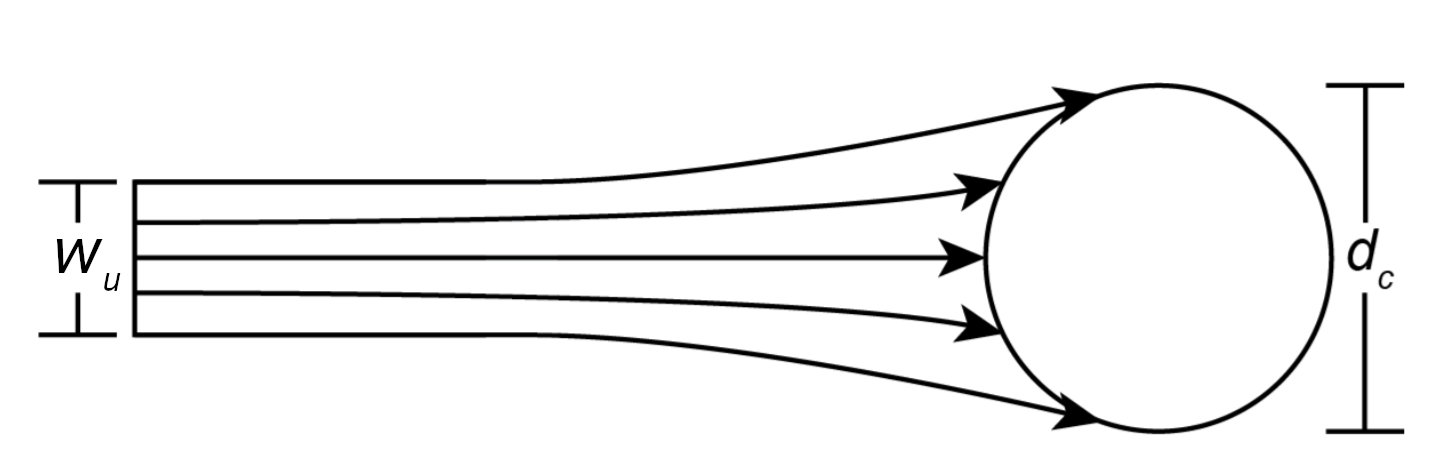
\includegraphics[width=5in]{../pics/collectorefficiency.png}
\centering
\caption{A diagram illustrating capture efficiency for a cylindrical collector. $b$ is the horizontal width of upstream flow and $d_c$ is collector diameter. Adapted from Palmer et al. (2004) \cite{Palmer_2004}.}
\label{fig:capeff}
\end{figure}

\section{Materials and Methods}

\subsection{Experimental Methods}

We conducted our experiments in the Ecogeomorphology flume, an indoor (temperature: $22.2$ +/- 1 \SI{}{\celsius}) recirculating flume located in McCone Hall at the University of California, Berkeley. The flume has a 5.25 m L $\times$ 0.6 m W $\times$ 0.6 m H open-channel section with a cuboid geometry and a bed and sidewalls that are smooth and transparent (Figure \ref{fig:floorplan}). At its upstream and downstream ends, this section connects to rectangular ducts with gradually changing hydraulic diameter and rounded corners with curved vertical manifolds along streamlines, both intended to maintain laminar flow. Additionally, at the upstream end of the open-channel, a honeycomb flow collimator serves to further straighten flow streamlines before the test section. The ducts in turn connect to the inlet and outlet of a special type of electric pump (Discflo Pumps Corporation Inc., Santee, CA), which uses rotating discs to entrain fluid and suspended particles through its interior chamber via viscous drag, maintaining laminar flow and avoiding alteration of particle or fluid properties (e.g., abrasion, pulsation) \cite{discflo}. Altogether, the flume design maintains constant, adjustable discharge through the open channel, minimizing background turbulence and other artifacts that arise with other types of pumps.

% Flume diagram figure
\begin{figure}[H]
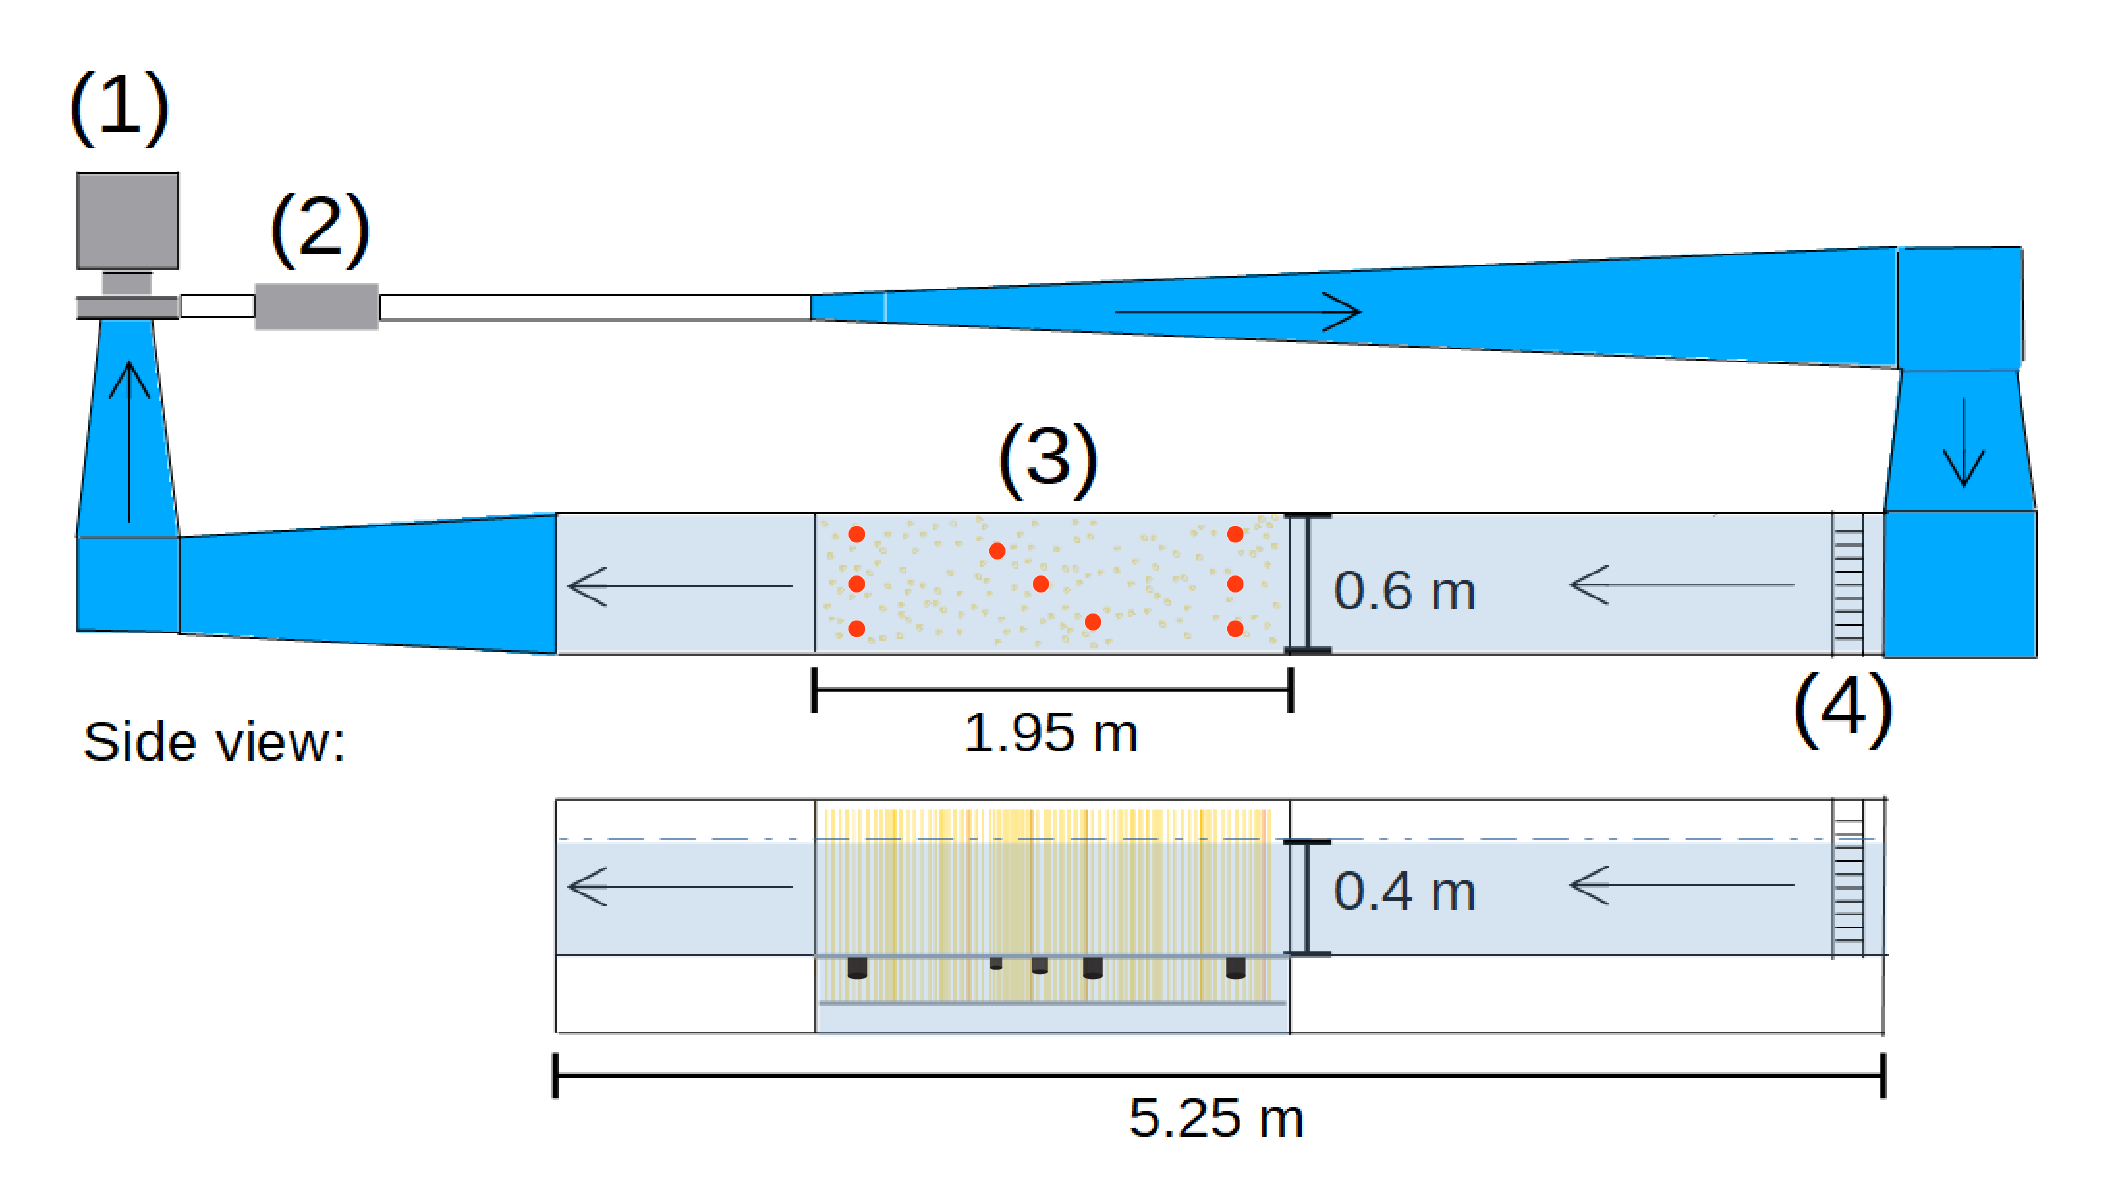
\includegraphics[width=5in]{../pics/flume_with_sedtraps.png}
\centering
\caption{The Ecogeomorphology flume. Not all measurements are to scale. \textbf{(a)} Photograph of the test section (left-center) and pump (right). \textbf{(b)} Conceptual diagram of the flume as seen from above. Labeled parts are: 1) pump, 2) magnetic flowmeter, 3) test section, and 4) honeycomb flow collimator. Arrows indicate direction of flow. Green points represent the inlets for the peristaltic pumps sampling suspended particle concentration. Red areas represent the sediment traps. \textbf{(c)} A side view of the open-channel part of the system.}
\label{fig:floorplan}
\end{figure}

Within the open-channel part of the flume, we designated a "test section" 1.95 m in length where collectors would be installed. This test section and the surrounding area were instrumented with the following devices:
\begin{enumerate}
     \item A flat-bedded array positioned flush with the neighboring channel bed, containing vertical, emergent collector stems, which were spaced uniformly in an unpatterned manner
    \item Two battery-operated peristaltic pumps (Cole-Parmer, Vernon Hills, IL) used to sample suspended particle concentration via three hose inlets each (inside diameter = 3.1 mm), which were suspended at a range of heights from the channel bed (5; 14; 27 cm); these were positioned both upstream and downstream of the test section 
   \item Sediment traps (n = 9) with 2.5 cm circular openings flush with the bed and collection filters recessed 5 cm below, which were used to estimate settled particle mass; these were interspersed among the collectors in a pattern intended to evaluate consistency throughout the test section
\end{enumerate}

We conducted experimental runs for a fully-crossed parameter space of collector Reynolds number (67; 134; 200) and collector density (0; 278; 800; 1450 collectors/m$^2$). These values, as well as other constant experimental parameters, were chosen to correspond to those that might occur for emergent grasses or reeds in natural settings (Table \ref{tbl:parameters}). A zero-collector control density was included in order to isolate the effects of our experimental installations from the background effects of the rest of the flume. We used 1/8" (0.3175 cm) cylindrical wooden dowels as collectors, which were covered in silicone grease (Chemplex 710, Fuchs Petrolub, Mannheim, Germany) in order to retain impacted particles. 

% Experimental parameters table
\begin{table}[H]
\caption{Experimental and natural parameter ranges. Natural values are based on approximations or measurements from cited studies and literature reviews.}
\centering
\begin{threeparttable}
\begin{tabular}{lcccc}
\toprule
\textbf{Parameter}&\textbf{This study}&\textbf{Fauria et al. (2015)}&\textbf{Purich (2006)}&\textbf{Natural}\\
\midrule
Flow velocity (\SI{}{\centi\metre/\second})     
& 2.0--6.0    & 1.8--6.1    & 1.0--10.2    & 0--25 \cite{nikora2008hydraulic}    \\
Flow depth (\SI{}{\centi\metre})                
& 40          & 14--17      & 12           & 0--50 \cite{kadlec1990}    \\
\midrule
Collector shape
& Cylindrical & Artificial grass  & Cylindrical & --- \\ 
Collector diameter (\SI{}{\centi\metre})
& 0.318       & 0.3         & 0.6          & 0.1--1.2 \cite{Nepf_2012,wright2018hydrological} \\
Collector Reynolds number                       
& 66--200     & 54--183     & 70--640      & 5--1000 \cite{kadlec1990}  \\ 
Collector density ($\#/\text{m}^2$)
& 278--1450   & 2724--7209  & 1013--4053   & 10--2700 \cite{wright2018hydrological} \\
Solid volume fraction (\%)
& 0.22--1.17  & 0.82--2.16  & 2.86--11.5   & 0.1--45 \cite{Nepf_2012} \\ 
\midrule
Particle type
& Walnut shell  & Road dust  & Pliolite\textsuperscript{\textregistered}   & --- \\ 
Specific gravity      
& 1.53        &2.27--2.61 \tnote{1}  & 1.03         & 2.56--2.87 \cite{czuba2015sedgravity} \\
Average particle diameter, $d_{50}$ (\SI{}{\micro\metre})     
& 25.2        & $\sim$10--15      & 212--250     & 45--100 \cite{hejduk2010variations,noe2010glades}  \\
Suspended concentration (\SI{}{\micro\liter/\liter})      
& 5.3--53.8   & 9--50       & $\sim$110   & 2-25 \cite{noe2010glades,aiona2013can}      \\
\midrule
Particle-collector diameter ratio, $R$      
&0.0079       &0.0004--0.083 \tnote{2} & 0.037        & <0.25     \\
\bottomrule
\vspace{-4mm}
\end{tabular}
\begin{tablenotes}
\footnotesize \item[1] Estimates from an observational study about road dust \cite{mckenzie2008size} (study-specific data unavailable)
\vspace{2mm}
\footnotesize \item[2] Fauria et al. \cite{Fauria_2015} used a LISST to measure collection across a broad range of particle diameters (1.25--250 \SI{}{\micro\metre})
\end{tablenotes}
\end{threeparttable}
\label{tbl:parameters}
\end{table}

Before each experiment, the flume was filled with tap water to 0.4 m depth in the test section, enough to completely fill the ducts and pump.

\subsection{Sediment Transport and Particle Capture Model}

\section{Results}

\subsection{Particle Capture}

Effective collector efficiency was found to decrease with increasing collector Reynolds number and collector density in nearly all cases (Figure \ref{fig:ece}). One exception occurred at the lowest collector density ($\phi_c = 0.22\%$), where the intermediate $\Rey_c$ treatment ($\Rey_c = 134$) had lower ECE than both the lower and higher $\Rey_c$ treatments (Figure \ref{fig:ece}a). When compared to the other collector-density treatments with the same $\Rey_c$ value, this low collector-density experiment's calculated ECE was slightly lower than the intermediate collector-density treatment, and was greater than the highest collector-density treatment (Figure \ref{fig:ece}b). For both of these comparisons, the large magnitude of our uncertainty leaves open the possibility that the mid-$\Rey_c$, low-collector-density result could simply be an anomaly.

% ECE figure
\begin{figure}[H]
\centering
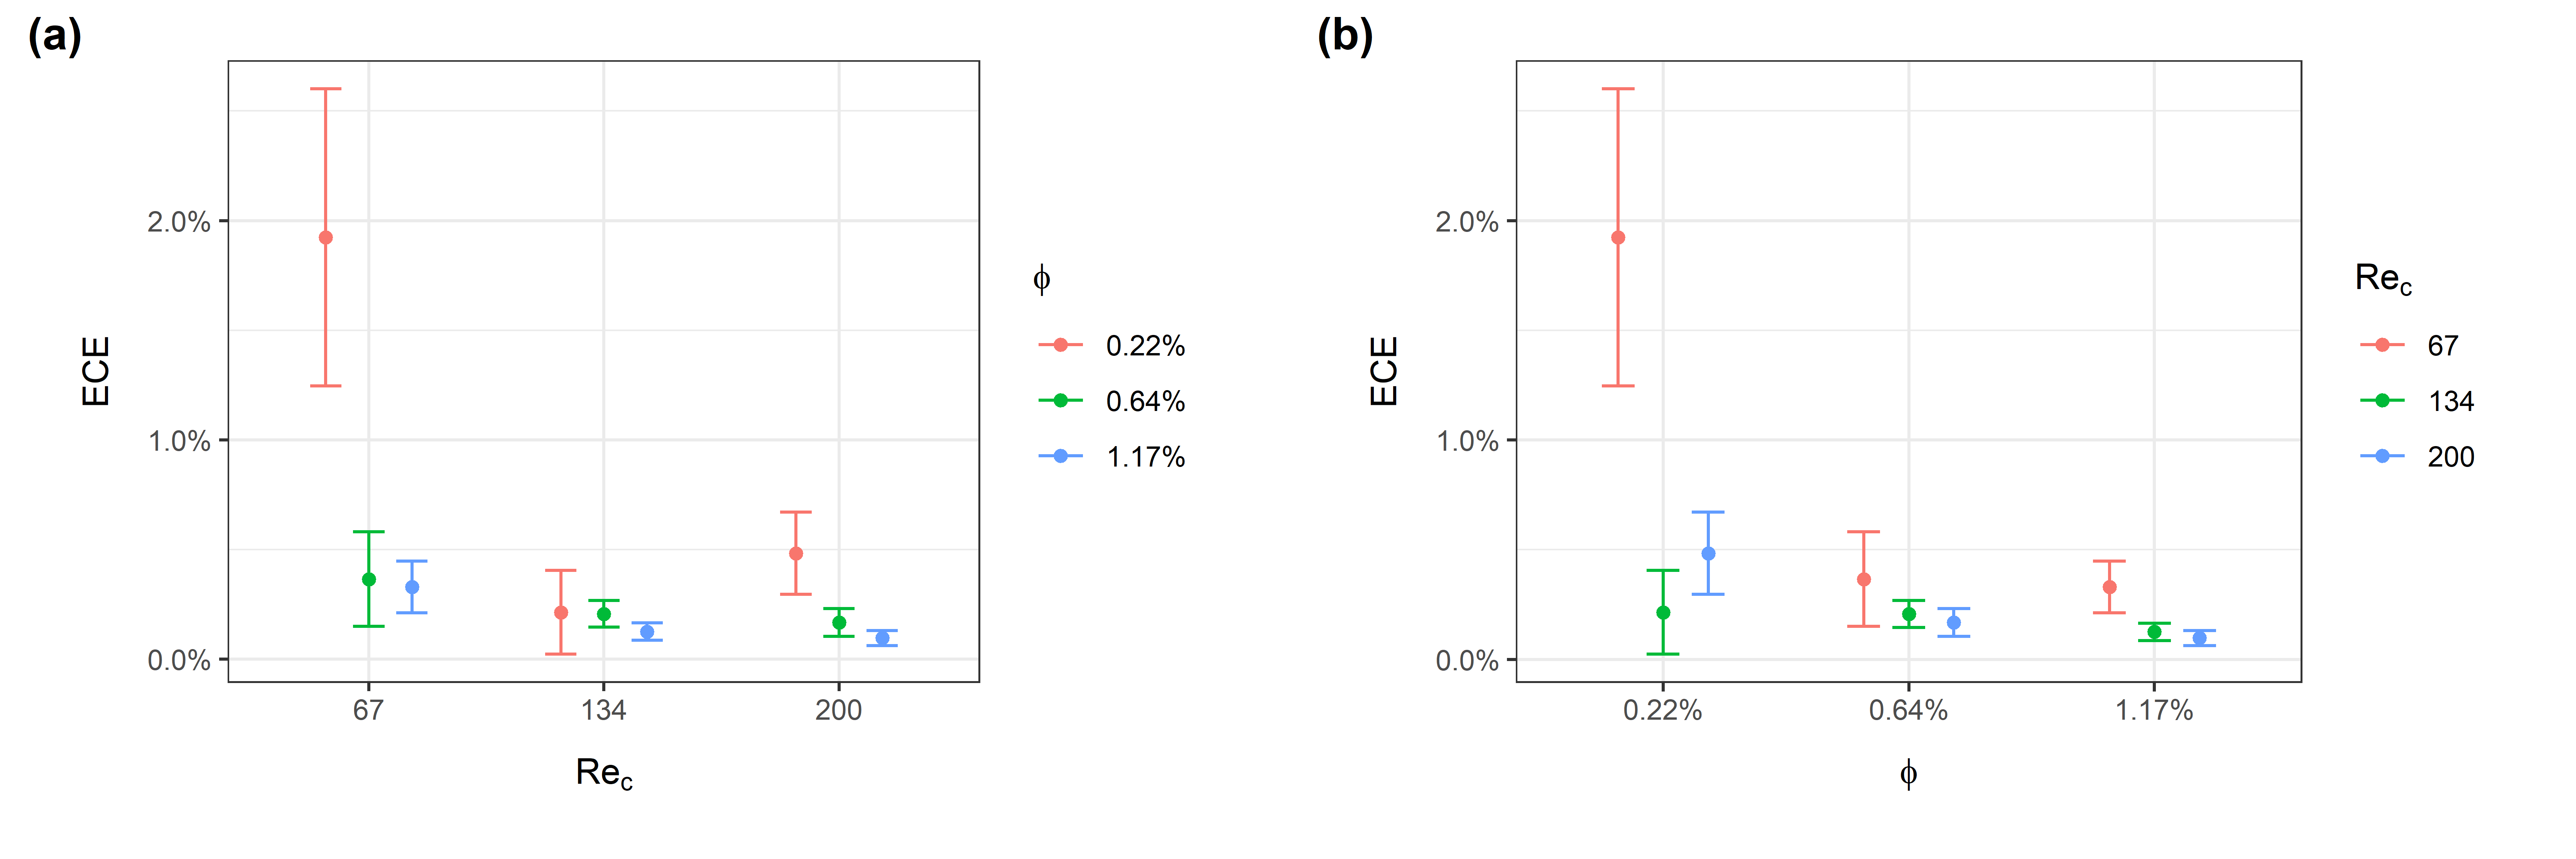
\includegraphics[width=5in]{../pics/ece_plot.png}
\caption{Estimates of effective capture efficiency calculated from laboratory experiments across the collector density $\times$ Reynolds number parameter space. Error bars represent +/- 1 SE. (\textbf{a}) Estimates plotted over $\Rey_c$, colored by solid volume fraction ($\phi_c$). (\textbf{b}) Estimates plotted over solid volume fraction, colored by $\Rey_c$.}
\label{fig:ece}
\end{figure}   

Monte Carlo analysis determined that there is a significant (null hypothesis: $\mu = 0$) negative relationship between ECE and collector density for the low (p = 0.004) and high (p = 0.019) $\Rey_c$ treatments, but no significant effect was detected (p > 0.05) for the intermediate treatment (Figure \ref{fig:monte}a). This approach also found a significant negative relationship between ECE and $\Rey_c$ for the low (p = 0.026) and high (p = 0.046) collector-density treatments, but an insignificant (p > 0.05) trend for the intermediate collector-density treatment (Figure \ref{fig:monte}b). 

% Monte Carlo figure
\begin{figure}[H]
\centering
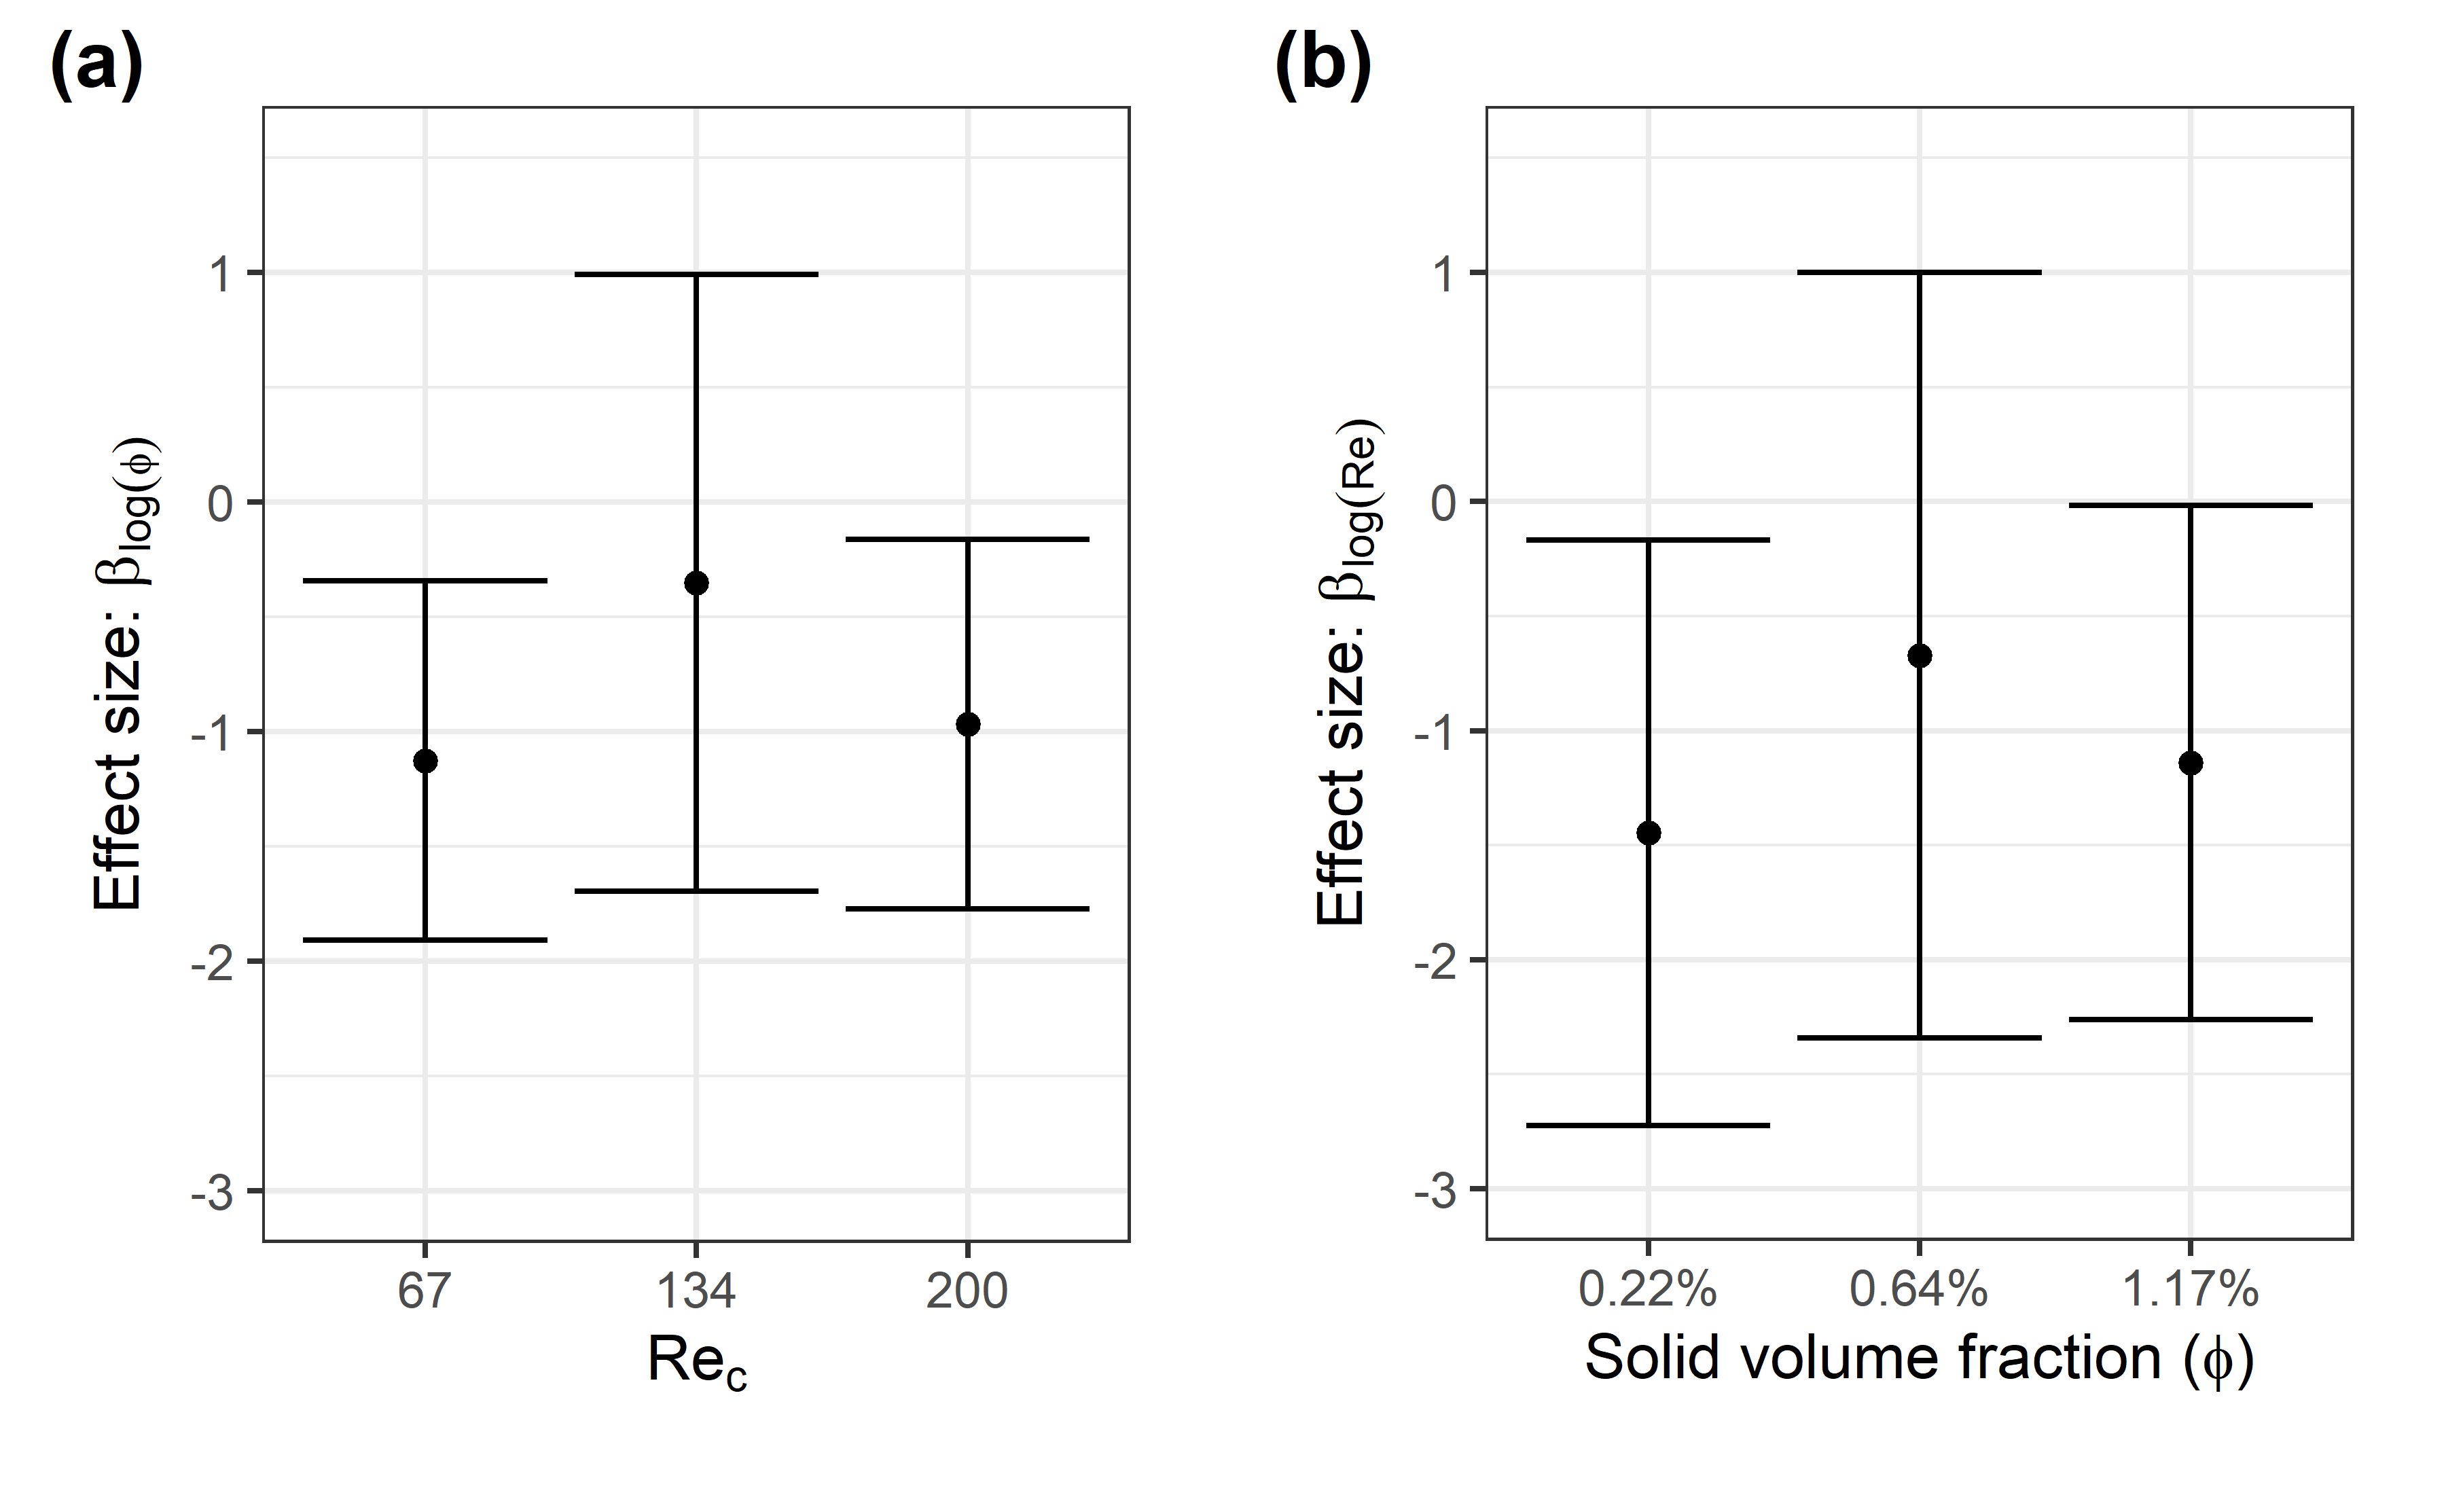
\includegraphics[width=5in]{../pics/montecarlo.png}
\caption{Effect size estimates resulting from Monte Carlo regression analysis. Error bars represent 95\% confidence intervals. Asterisks mark the parameter values at which the effect size was found to be significant (\textbf{a}) Estimates of the effect of log-transformed collector solid volume fraction ($\beta_{\log(\phi_c)}$) on ECE, stratified by $\Rey_c$. (\textbf{b}) Estimates of the effect of log-transformed $\Rey_c$ ($\beta_{\log(\Rey_c)}$) on ECE, stratified by solid volume fraction ($\phi_c$).}
\label{fig:monte}
\end{figure}   

\subsection{Turbulence and Flow Characteristics}

% Turbulence table
\begin{table}[H]
\caption{Turbulence and flow characteristics for all collector solid volume fraction ($\phi_c$) and $\Rey_c$ treatments, including the control (zero-collector) treatments for reference.}
\centering
%% \tablesize{} %% You can specify the fontsize here, e.g., \tablesize{\footnotesize}. If commented out \small will be used.
\begin{tabular}{>{\bfseries}r>{\bfseries}rrr}
\toprule
\textbf{$\phi_c$}&\textbf{$\Rey_c$}&\textbf{Turbulent Kinetic Energy (\SI{}{\metre^2/\second^2})}\\
\midrule
Control &   67  & \num{2.48d-6}\\
        &   134 & \num{2.98d-6}\\
        &   200 & \num{3.37d-6}\\
\midrule
0.22\% &   67  & \num{1.23d-6}\\
        &   134 & \num{5.26d-6}\\
        &   200 & \num{1.22d-5}\\
\midrule
0.64\% &   67  & \num{9.13d-6}\\
        &   134 & \num{3.59d-5}\\
        &   200 & \num{5.96d-5}\\
\midrule
1.17\%  &   67  & \num{1.11d-5}\\
        &   134 & \num{2.98d-5}\\
        &   200 & \num{5.44d-5}\\
\bottomrule
\label{tbl:turbulence}
\end{tabular}
\end{table}

\subsection{Biofilm Effects}

% Biofilm figure
\begin{figure}[H]
\centering
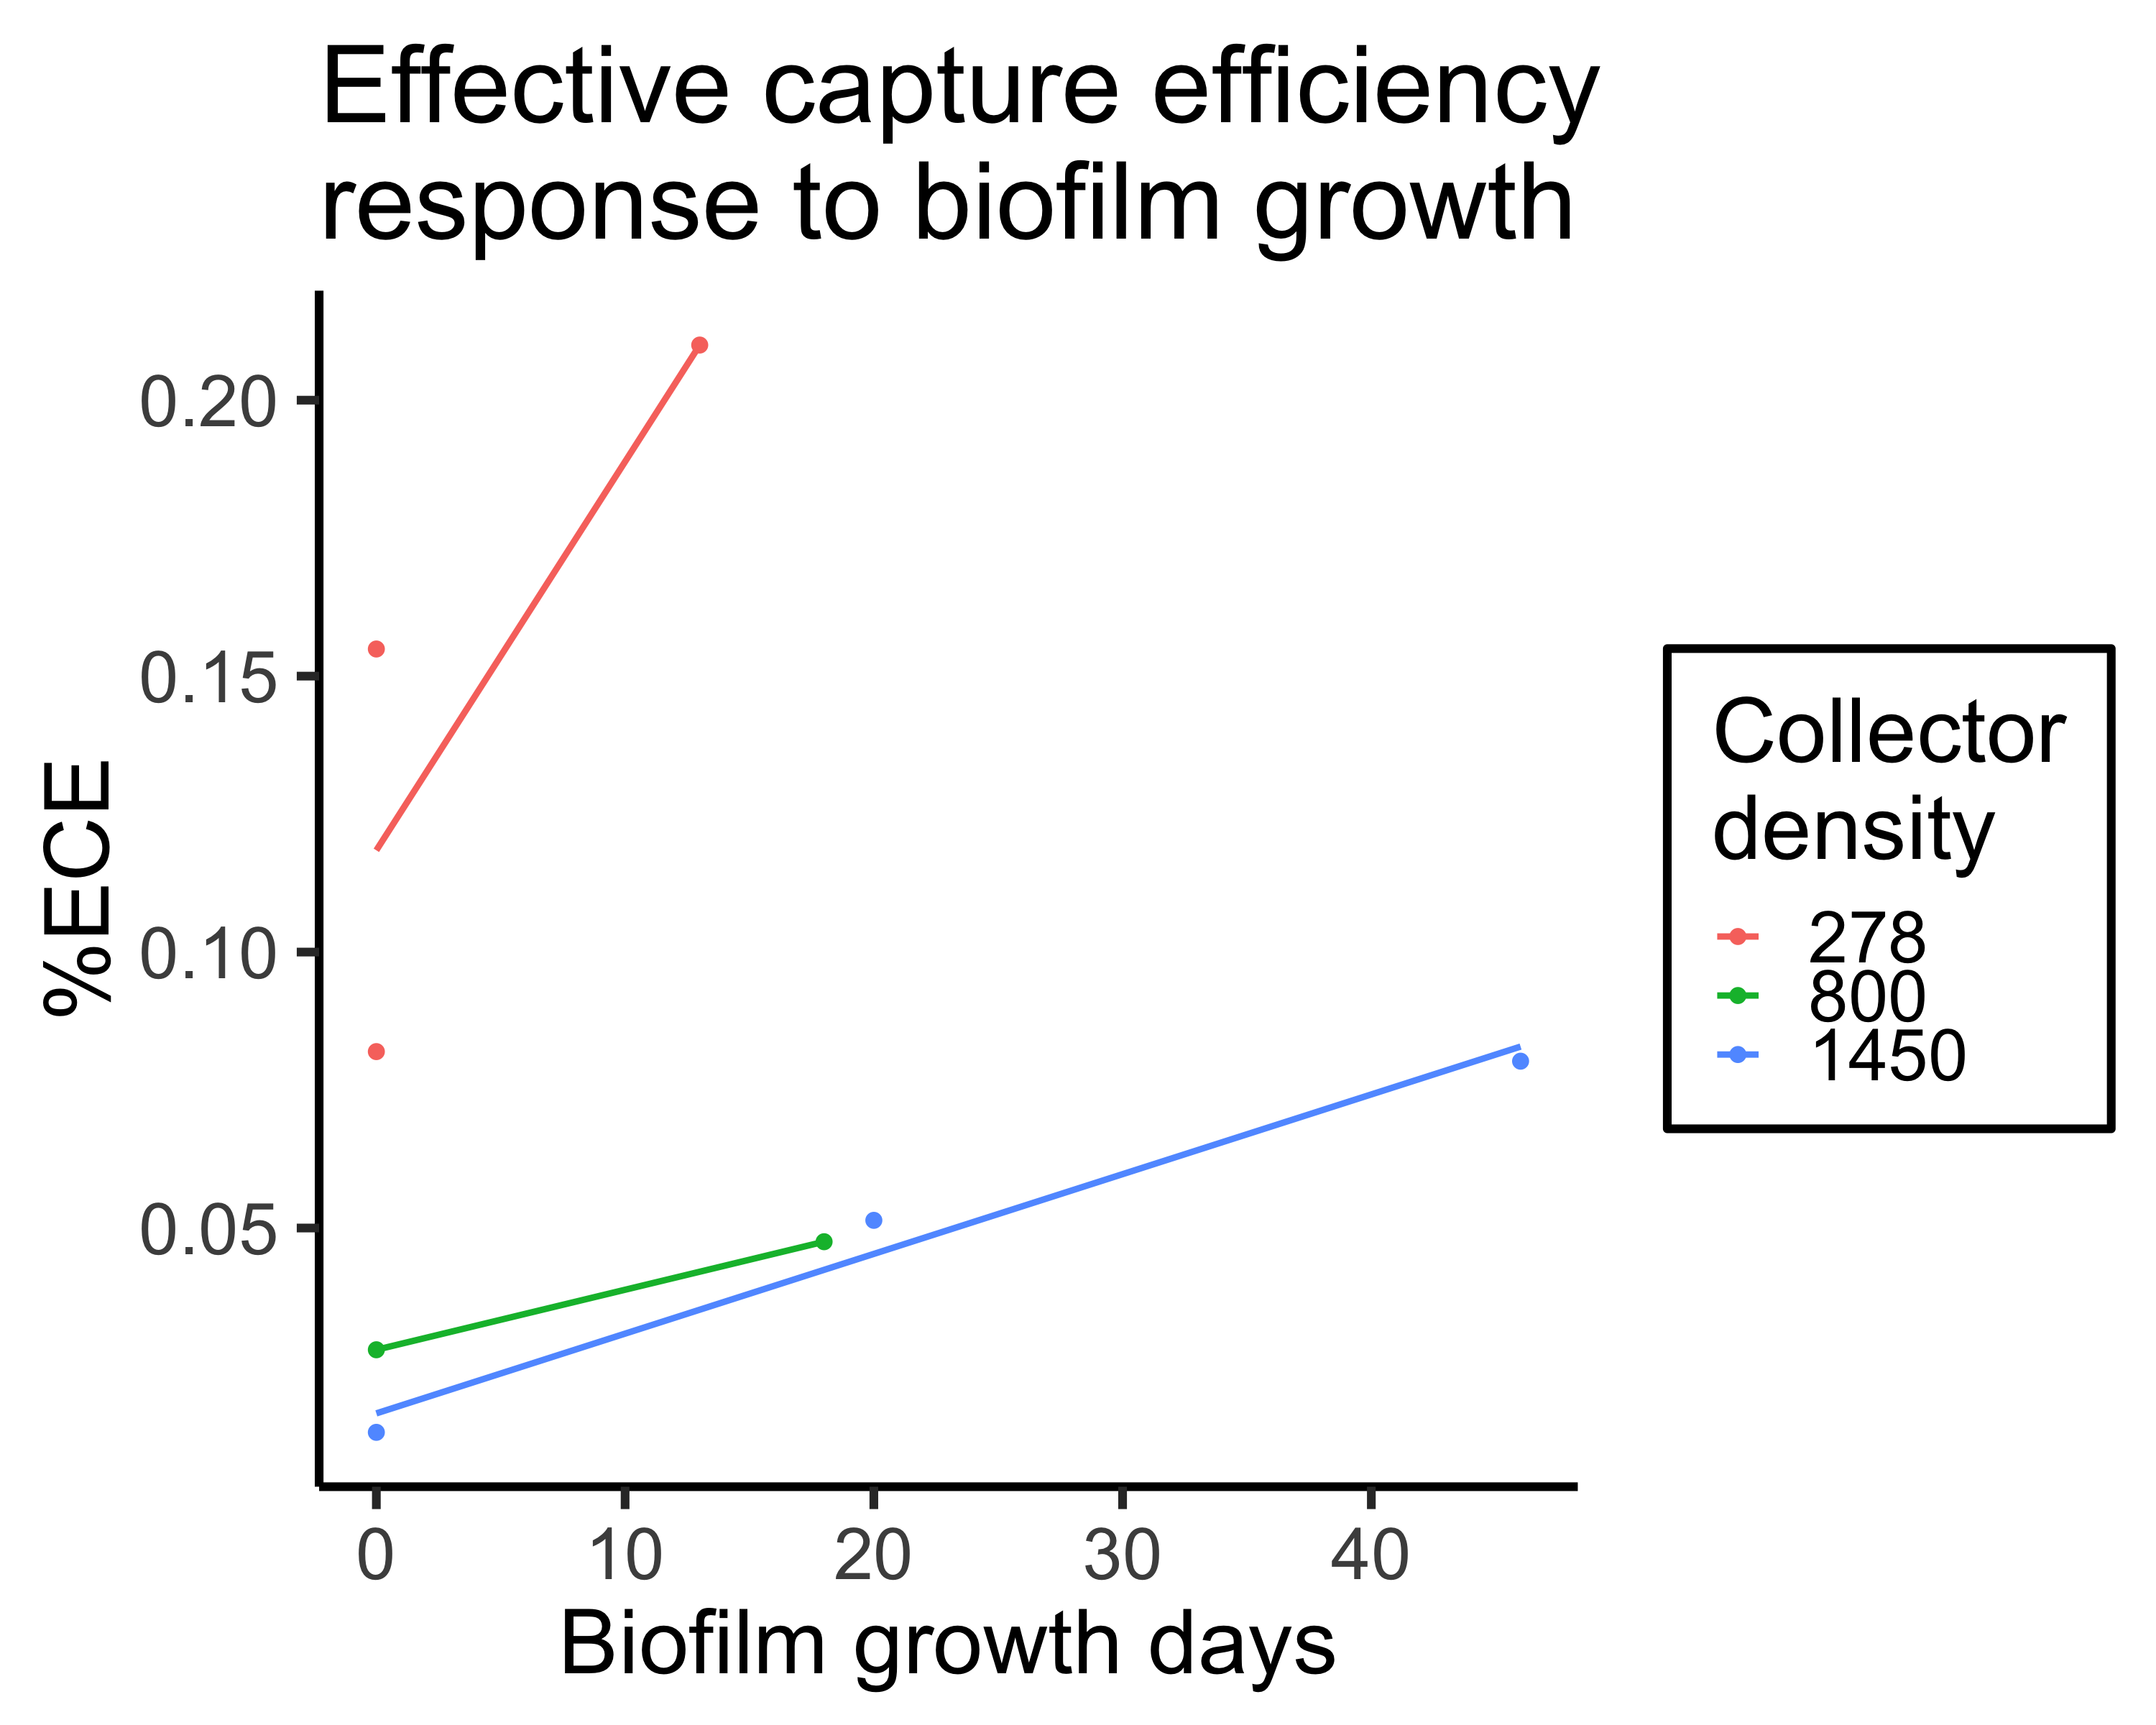
\includegraphics[width=5in]{../pics/biofilm.png}
\caption{Estimates of effective capture efficiency calculated from experimental runs with varying degrees of biofilm growth. Colors represent the different collector densities, expressed as solid volume fraction ($\phi_c$). Straight lines are drawn between the points that represent our experiments and the shaded areas represent 95\% confidence intervals for ECE inferred from our measurement uncertainty.}
\label{fig:biofilm}
\end{figure}   

\subsection{Comparison to Previous Models of Capture Efficiency}

% Fauria model comparison figure
\begin{figure}[H]
\centering
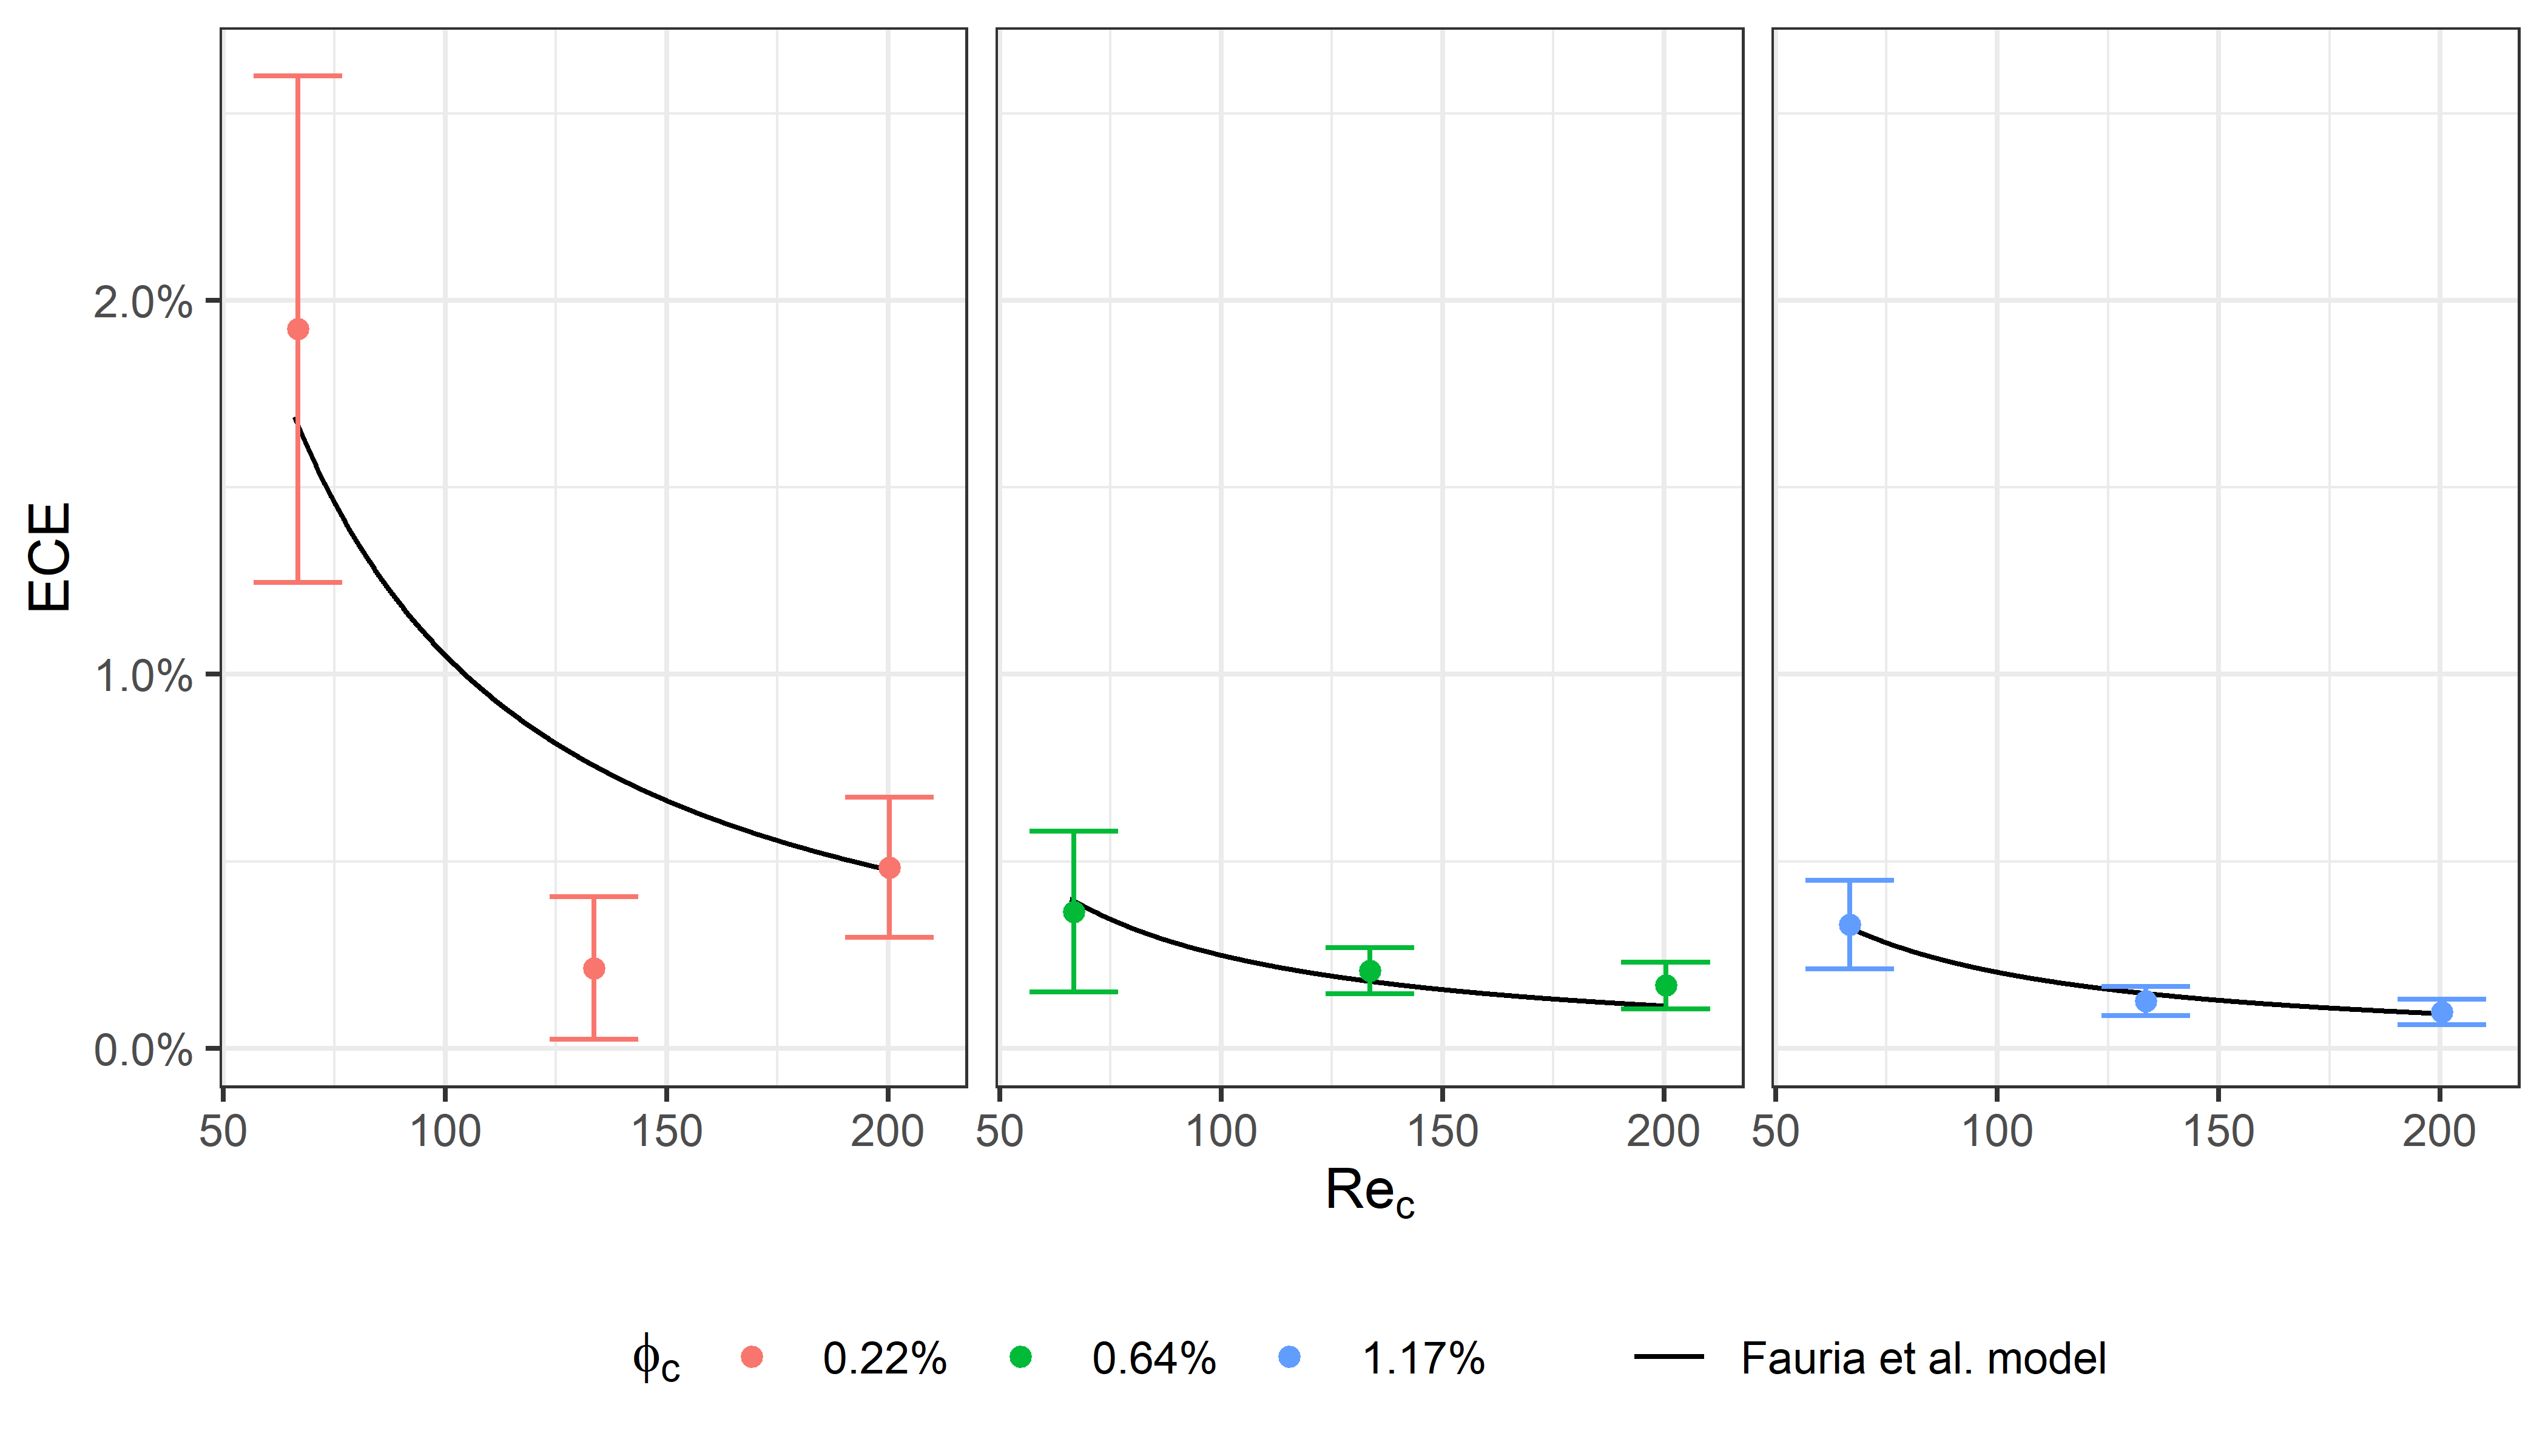
\includegraphics[width=5in]{../pics/comparisonplot.png}
\caption{A comparison of our experimental estimates of effective capture efficiency, colored according to collector solid volume fraction ($\phi_c$), and the predictions of the Fauria et al. \cite{Fauria_2015} power law model. Effective capture efficiency is plotted on a log scale in order to display model fit more accurately at small values. Error bars represent +/- 1 SE.}
\label{fig:compplot}
\end{figure}   

% C-phi model figure
\begin{figure}[H]
\centering
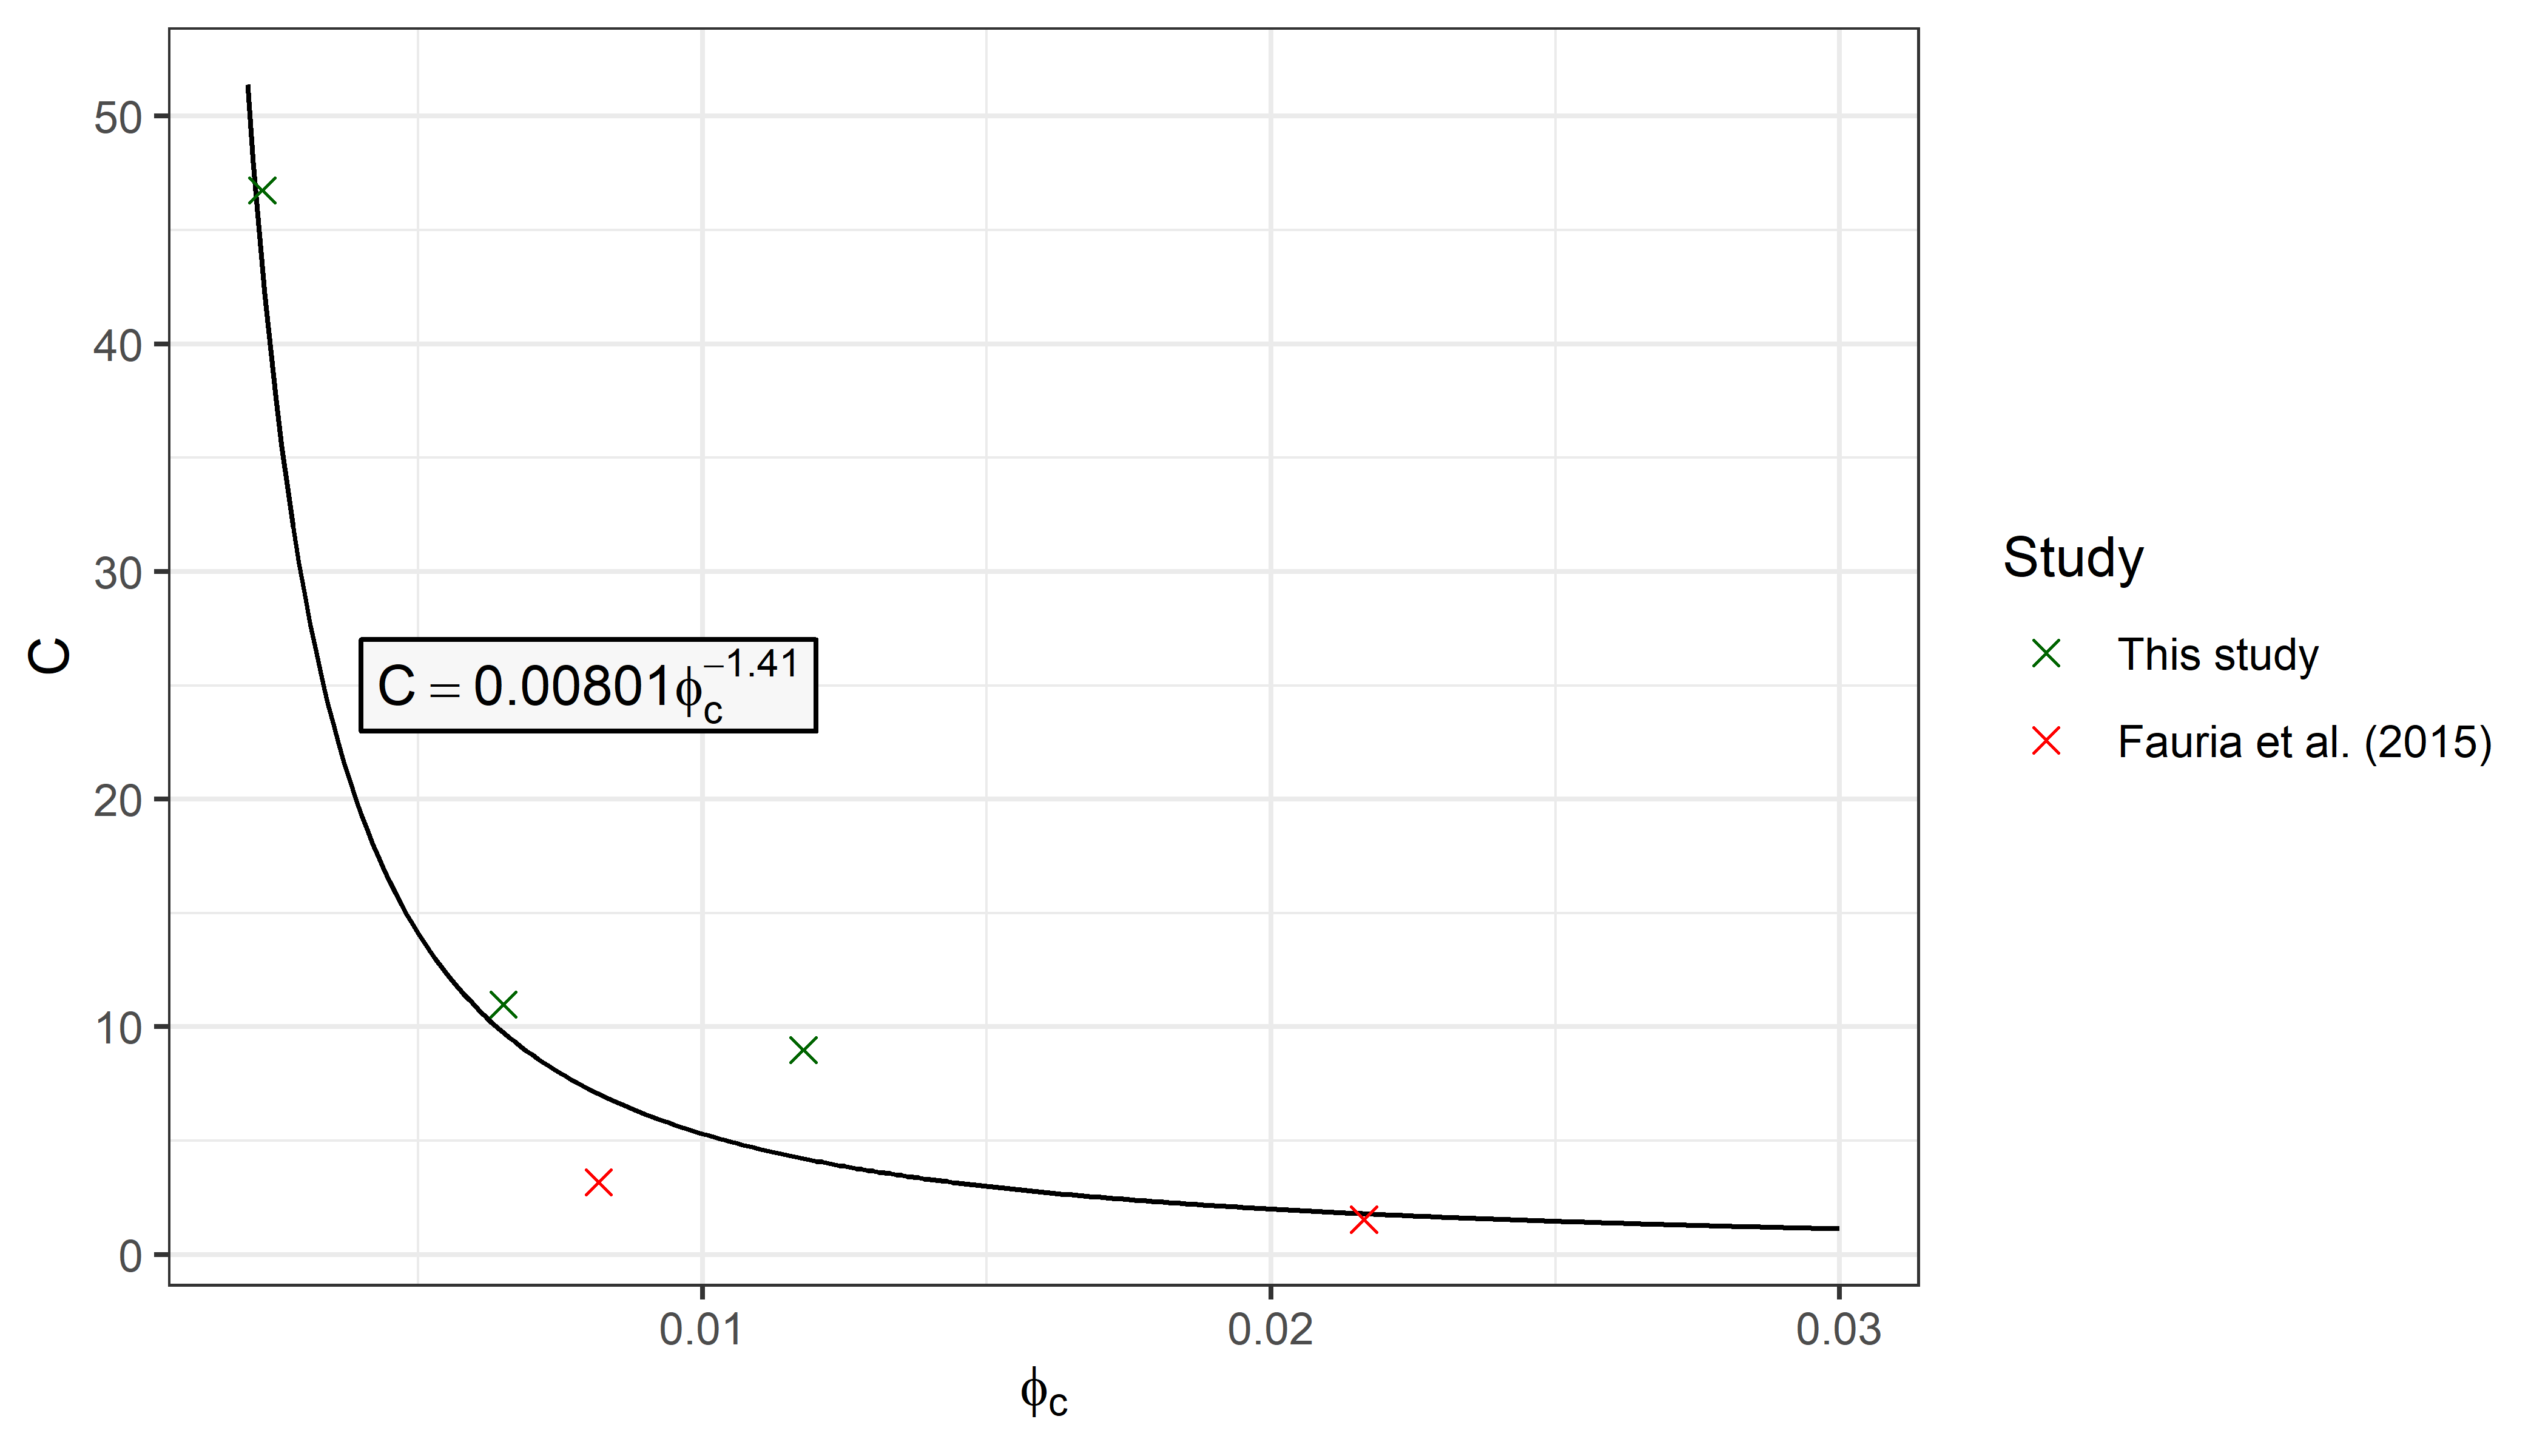
\includegraphics[width=5in]{../pics/cphiplot.png}
\caption{A comparison of the $C$ values calculuated for each of our collector-density treatments to those calculated by Fauria et al. \cite{Fauria_2015}. The black line represents the power law model of best fit between $C$ and collector solid volume fraction ($\phi_c$) for our collector-density treaments and those of Fauria et al. combined (n = 5), for which R$^2$ = 0.82.}
\label{fig:cphi}
\end{figure}   

\section{Discussion}

\subsection{Inferred Mechanisms of Effect for Collector Density and Reynolds Number}

\subsection{Relative Importance of Biofilm}

\subsection{Designing Wetlands for Maximum Sedimentation}

\vspace{6pt} 

%%%%%%%%%%%%%%%%%%%%%%%%%%%%%%%%%%%%%%%%%%
%% optional
%\supplementary{The following are available online at \linksupplementary{s1}, Figure S1: title, Table S1: title, Video S1: title.}

% Only for the journal Methods and Protocols:
% If you wish to submit a video article, please do so with any other supplementary material.
% \supplementary{The following are available at \linksupplementary{s1}, Figure S1: title, Table S1: title, Video S1: title. A supporting video article is available at doi: link.}

\authorcontributions{Conceptualization, L.L., J.N., and J.W.; methodology, L.L. and J.W.; software, L.L., J.N., J.W., and C.Y.; validation, J.W.; formal analysis, J.W. and C.Y.; investigation, J.N., J.W, and C.Y.; resources, L.L.; data curation, J.W.; writing--original draft preparation, J.N., J.W., and C.Y.; writing--review and editing, L.L., J.N., J.W., and C.Y.; visualization, J.W.; supervision, L.L., J.W., and C.Y.; project administration, L.L. and J.W.; funding acquisition, L.L.}

\funding{This research was funded by NSF award \#1455362.}

\acknowledgments{The authors wish to thank and acknowledge Colin Keating and Aaron Hurst for their helpful work on preliminary flume experiments. We also wish to express great thanks to Yayla Sezinger, Elle Chen, Nicole Ulakovic, Katrina Ginsberg, and Danielle Satin for their time spent preparing for experiments, maintaining the flume, and fastidiously carrying out other important laboratory tasks. Lastly, we wish to thank Sam Stein and Sheila Trampush for graciously sharing data and participating in brainstorming sessions while working on concurrent studies within the same general topic area.}

\conflictsofinterest{The authors declare no conflict of interest.} 

%% optional
% \abbreviations{The following abbreviations are used in this manuscript:\\

% \noindent 
% \begin{tabular}{@{}ll}
% MDPI & Multidisciplinary Digital Publishing Institute\\
% DOAJ & Directory of open access journals\\
% TLA & Three letter acronym\\
% LD & linear dichroism
% \end{tabular}}

%%%%%%%%%%%%%%%%%%%%%%%%%%%%%%%%%%%%%%%%%%
%% optional
% \appendixtitles{no} %Leave argument "no" if all appendix headings stay EMPTY (then no dot is printed after "Appendix A"). If the appendix sections contain a heading then change the argument to "yes".
% \appendix
% \section{}
% \unskip
% \subsection{}
% The appendix is an optional section that can contain details and data supplemental to the main text. For example, explanations of experimental details that would disrupt the flow of the main text, but nonetheless remain crucial to understanding and reproducing the research shown; figures of replicates for experiments of which representative data is shown in the main text can be added here if brief, or as Supplementary data. Mathematical proofs of results not central to the paper can be added as an appendix.

% \section{}
% All appendix sections must be cited in the main text. In the appendixes, Figures, Tables, etc. should be labeled starting with `A', e.g., Figure A1, Figure A2, etc. 

%%%%%%%%%%%%%%%%%%%%%%%%%%%%%%%%%%%%%%%%%%
% Citations and References in Supplementary files are permitted provided that they also appear in the reference list here. 

%=====================================
% The following MDPI journals use author-date citation: Arts, Econometrics, Economies, Genealogy, Humanities, IJFS, JRFM, Laws, Religions, Risks, Social Sciences. For those journals, please follow the formatting guidelines on http://www.mdpi.com/authors/references
% To cite two works by the same author: \citeauthor{ref-journal-1a} (\citeyear{ref-journal-1a}, \citeyear{ref-journal-1b}). This produces: Whittaker (1967, 1975)
% To cite two works by the same author with specific pages: \citeauthor{ref-journal-3a} (\citeyear{ref-journal-3a}, p. 328; \citeyear{ref-journal-3b}, p.475). This produces: Wong (1999, p. 328; 2000, p. 475)

% =====================================
% References, variant B: external bibliography
% =====================================

\reftitle{References}
\externalbibliography{yes}
\bibliography{refs}

%%%%%%%%%%%%%%%%%%%%%%%%%%%%%%%%%%%%%%%%%%
%% optional
%\sampleavailability{Samples of the compounds ...... are available from the authors.}

%% for journal Sci
%\reviewreports{\\
%Reviewer 1 comments and authors’ response\\
%Reviewer 2 comments and authors’ response\\
%Reviewer 3 comments and authors’ response
%}

%%%%%%%%%%%%%%%%%%%%%%%%%%%%%%%%%%%%%%%%%%

\end{document}
